\section{Pengantar Op Amp}

\begin{frame}{Pengantar Op Amp}
\begin{figure}
	\centering
	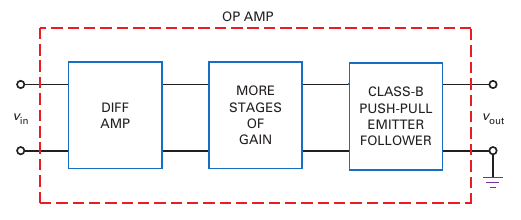
\includegraphics[width=0.8\linewidth]{gambar/fig-16.01}
	\caption{Blok diagram sebuah op amp}
	\label{fig-16.01}
\end{figure}
\end{frame}

\begin{frame}{Pengantar Op Amp}
	\begin{itemize}
		\item Gambar \ref{fig-16.01} adalah diagram blok dari sebuah op amp.
		\item Input stage-nya adalah diff amp, kemudian diikuti dengan lebih banyak tahapan-tahapan penguat dan sebuah Class-B push-pull emitter follower.
		\item Karena diff amp adalah tahapan pertamanya maka hal ini yang menentukan karakteristik input dari op amp.
		\item Sebagian besar op amp adalah single-ended output, seperti pada Gambar \ref{fig-16.01}.
		\item Dengan supply positif dan negatif, single-ended output dirancang untuk memiliki nilai quiescent/ nilai diam sebesar nol.
	\end{itemize}
\end{frame}

\begin{frame}{Pengantar Op Amp}
	\begin{itemize}
		\item Tidak semua op amp dirancang seperti Gambar \ref{fig-16.01}.
		\item Beberapa op amp tidak menggunakan Class-B push-pull output, dan ada juga yang memiliki double-ended output.
		\item Op amp juga tidak sesederhana seperti pada Gambar \ref{fig-16.01}.
		\item Rancangan internal dari monolithic op amp sangat rumit, menggunakan ribuan transistor sebagai current mirrors, active load, dan inovasi lainnya yang tidak mungkin di dalam rancangan diskret.
		\item Gambar \ref{fig-16.01} hanya menunjukkan 2 fitur penting yang umumnya digunakan di op amp, yaitu differential input dan single-ended output.
	\end{itemize}
\end{frame}

\begin{frame}{Pengantar Op Amp}
	\begin{figure}
		\centering
		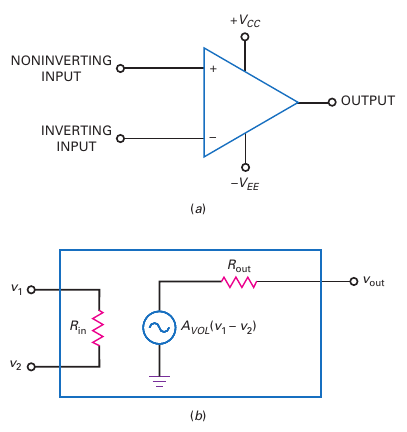
\includegraphics[width=0.4\linewidth]{gambar/fig-16.02}
		\caption{(a) Simbol dari op amp dan (b) rangkaian ekivalen dari op amp}
		\label{fig-16.02}
	\end{figure}
\end{frame}

\begin{frame}{Pengantar Op Amp}
	\begin{itemize}
		\item Gambar \ref{fig-16.02}a adalah simbol skematik dari sebuah op amp.
		\item Memiliki noninverting dan inverting input dan single-ended output.
		\item Idealnya, simbol ini menunjukkan amplifier memiliki voltage gain tak hingga, impedansi input tak hingga, dan nol impedansi input.
		\item Op amp ideal merepresentasikan voltage amplifier yang sempurna dan sering disebut sebagai voltage-controlled voltage source (VCVS).
		\item VCVS ditunjukkan oleh Gambar \ref{fig-16.02}b, dimana $ R_{in} $ bernilai tak hingga dan $ R_{out} $ bernilai nol.
	\end{itemize}
\end{frame}

\begin{frame}{Pengantar Op Amp}
	\begin{figure}
		\centering
		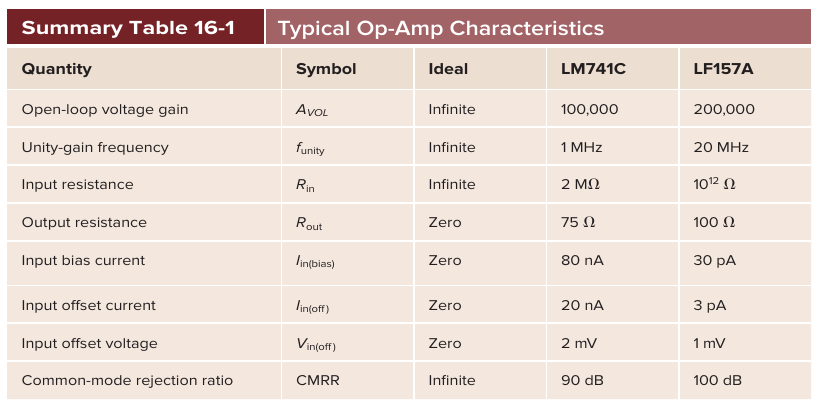
\includegraphics[width=0.8\linewidth]{gambar/tab-16.01}
		\caption{Perbandingan karakteristik op amp ideal dan op amp standar}
		\label{tab-16.01}
	\end{figure}
\end{frame}

\begin{frame}{Pengantar Op Amp}
	\begin{itemize}
		\item Tabel yang ditunjukkan oleh Gambar \ref{tab-16.01} adalah ringkasan dari karakteristik op amp ideal.
		\item Memiliki voltage gain, unity-gain frekuensi, input impedansi, dan CMRR yang bernilai tak hingga.
		\item Memiliki resistor ouput, arus bias, offset yang bernilai nol.
		\item Seperti itulah seharusnya manufaktur membuat op amp, jika mereka mampu.
		\item Namun kenyataannya mereka hanya mampu membuat yang mendekati nilai idealnya saja.
	\end{itemize}
\end{frame}

\begin{frame}{Pengantar Op Amp}
	\begin{itemize}
		\item LM741C memiliki voltage gain sebesar 100000, unity-gain frekuensi sebesar 1 MHz, dan impedansi input sebesar 2 M$ \Omega $, dan seterusnya.
		\item Karena voltage gain yang sangat besar, input offset dapat dengan mudahnya memenuhi op amp.
		\item Sehingga diperlukan komponen eksternal antara input dan output op amp untuk menstabilkan voltage gain.
		\item Contohnya, menggunakan negative feedback untuk menyesuaikan voltage gain keseluruhan menjadi ke nilai yang lebih kecil sebagai ganti operasi linier yang stabil.
	\end{itemize}
\end{frame}

\begin{frame}{Pengantar Op Amp}
	\begin{itemize}
		\item Ketika tidak ada jalur feedback yang digunakan, voltage gain bernilai maksimum yang disebut sebagai open-loop voltage gain, $ A_{VOL} $
		\item Pada Gambar \ref{tab-16.01}, $ A_{VOL} $ dari LM741C bernilai 100000.
		\item Meskipun bukan bernilai tak hingga, open-loop voltage gain ini sangat tinggi.
		\item Contohnya, sebuah input sekecil 10 $ \mu $V akan menghasilkan output sebesar 1 V.
		\item Karena open-loop voltage gain sangat besar, kita dapat menggunakan heavy negative feedback untuk meningkatkan performa keseluruhan rangkaian.
	\end{itemize}
\end{frame}

\begin{frame}{Pengantar Op Amp}
	\begin{itemize}
		\item 741C memiliki unity-gain frequency sebesar 1 MHz, artinya kita memperolah voltage gain hingga 1 MHz.
		\item 741C memiliki input resistance sebesar 2 M$ \Omega $, output resistance sebesar 75 $\Omega$, arus bias input sebesar 80 nA, arus offset input sebsar 20 nA, tegangan offset input sebesar 2 mV, dan CMRR sebesar 90 dB.
		\item Saat resistor yang lebih tinggi dibutuhkan, seorang designer dapat menggunakan op amp BIFET.
		\item JFET digunakan di input stage untuk mendapatkan input bias dan arus offset yang lebih kecil.
		\item Bipolar transistor digunakan pada stage selanjutnya untuk mendapatkan lebih banyak voltage gain.
	\end{itemize}
\end{frame}

\begin{frame}{Pengantar Op Amp}
	\begin{itemize}
		\item LF571A adalah contoh dari op amp BIFET.
		\item Seperti yang ditunjukkan oleh Gambar \ref{tab-16.01}, arus bias inputnya hanya 30 pA dan input resistance adalah $ 10^{12} ~\Omega$.
		\item Memiliki voltage gain 200000 dan unity-gain frequency sebesar 20 MHz.
		\item Dengan menggunakan op amp ini kita bisa mendapatkan voltage gain hingga 20 MHz.
	\end{itemize}
\end{frame}